% \documentclass[a4paper,10pt]{article} % or whatever
% \documentclass[letterpaper,10pt]{article} % or whatever
\documentclass{article}

% if you need to pass options to natbib, use, e.g.:
     \PassOptionsToPackage{numbers, compress}{natbib}
% before loading neurips_2020

% ready for submission
% \usepackage{neurips_2021}

% to compile a preprint version, e.g., for submission to arXiv, add add the
% [preprint] option:
% \usepackage[final]{neurips_2021}

% to compile a camera-ready version, add the [final] option, e.g.:

% \usepackage[final]{neurips_2020}
\usepackage[preprint]{neurips_2021}
% \usepackage[preprint]{neurips_2021}


% to compile a camera-ready version, add the [final] option, e.g.:


% \newtheorem*{notice}{Notice}

% \theoremstyle{definition}
% \newtheorem{dfn}[equation]{Definition}
% \newtheorem{bigrem}[equation]{Remark}
% \newtheorem{num}[equation]{} % a bit strange, but I do use it!
% \newtheorem{exmp}[equation]{Example}


\newcommand{\ignore}[1]{}
% to avoid loading the natbib package, add option nonatbib:
\usepackage{dsfont}
\input{preamble}
\usepackage{tikz}
\usetikzlibrary{shapes.geometric, arrows}
%  \usepackage{subfigure} 
\pdfminorversion=7

%\floatname{algorithm}{Procedure}
\renewcommand{\algorithmicrequire}{\textbf{Input:}}
\renewcommand{\algorithmicensure}{\textbf{Output:}}


\usepackage[utf8]{inputenc} % allow utf-8 input
\usepackage{microtype}      % microtypography

%\tikzstyle{input} = [rectangle, rounded corners, minimum width=1cm, minimum height=1cm,text centered, draw=black]
%\tikzstyle{process} = [rectangle, minimum width=3cm, minimum height=1cm, text centered, draw=black]
%\tikzstyle{output} = [rectangle, rounded corners, minimum width=1cm, minimum height=1cm,text centered, draw=black]
\title{Inequality and Approximate}
% \author{%
%   Qiyu~Kang, and Wee~Peng~Tay
%  \thanks{First two authors contributed equally to this work.} 
%   \\
%   School of Electrical and Electronic Engineering\\
%   Nanyang Technological University\\
%   Singapore \\
% %   \texttt{songy@ntu.edu.sg, kang0080@e.ntu.edu.sg, wptay@ntu.edu.sg, qding001@e.ntu.edu.sg} \\
%   % examples of more authors
%   % \And
%   % Coauthor \\
%   % Affiliation \\
%   % Address \\
%   % \texttt{email} \\
% }



\begin{document}

\maketitle

% \begin{abstract}

% Deep neural networks (DNNs) are well-known to be vulnerable to adversarial attacks, where malicious human-imperceptible perturbations are included in the input to the deep network to fool it into making a wrong classification. Recent studies have demonstrated that neural Ordinary Differential Equations (ODEs) are intrinsically more robust against adversarial attacks compared to vanilla DNNs. In this work, we propose a stable neural ODE with Lyapunov-stable equilibrium points for defending against adversarial attacks (SODEF). By ensuring that the equilibrium points of the ODE solution used as part of SODEF is Lyapunov-stable, the ODE solution for an input with a small perturbation converges to the same solution as the unperturbed input. We provide theoretical results that give insights into the stability of SODEF as well as the choice of regularizers to ensure its stability. Our analysis suggests that our proposed regularizers force the extracted feature points to be within a neighborhood of the Lyapunov-stable equilibrium points of the ODE. SODEF is compatible with many defense methods and can be applied to any neural network's final regressor layer to enhance its stability against adversarial attacks. 
% \end{abstract}
\section{Bernoulli's inequality}
\begin{enumerate}
    \item For every \textbf{integer} $r\ge 0$ and every real number $x\ge -1$. \begin{align}
        (1+x)^{r} \geq 1+r x \label{ber:1}
    \end{align}
    If the exponent $r$ is even, then the inequality is valid for all real numbers $x$.
    \item For every \textbf{integer} $r \geq 2$ and every real number $x \geq-1$ with $x \neq 0$. \begin{align}
        (1+x)^{r}>1+r x. \label{ber:2}
    \end{align}
    \item For every \textbf{real number} $r \geq 1$ and real number $x \geq-1$, \begin{align}
        (1+x)^{r} \geq 1+r x. \label{ber:3}
    \end{align}
    \item For $0 \leq r \leq 1$ and \textbf{real number} $x \geq-1$, \begin{align}
        (1+x)^{r} \leq 1+r x. \label{ber:4}
    \end{align}
    \item Above give the lower bound (except \cref{ber:4}), here we get an upper bound,  for any real numbers $x, r$ with $r> 0$, \begin{align}
        (1+x)^{r}\leq e^{rx}.\label{ber:5}
    \end{align}
    \begin{proof}
    From Rudin\cite{rudin1976principles} we know $\lim_{k\to\infty}(1+1/k)^k=e$ and from \href{https://math.stackexchange.com/questions/167843/show-that-left1-dfrac1n-rightn-is-monotonically-increasing}{the link here} we know $(1+1/k)^k$ increases with positive $k$, we thus have
    \begin{align}
        (1+1/k)^k<e \label{ber:5a}
    \end{align} for positive integer $k$. Hence $(1+x)^{r}=\left((1+x)^{1/x}\right)^{xr}\le e^{rx}$ for $x>0$. Similarly we have $(1+1/k)^k$ increases with negative $k$ and $(1+1/k)^k>e$ for negative $k$. Hence $(1+x)^{r}=\left((1+x)^{1/x}\right)^{xr}\ge e^{rx}$ for $x<0$.
    \end{proof}
    \item $\left|\log (1+x)-x \right|\le x^2$ if  $|x|< 1/2$
\end{enumerate}

\begin{figure}[ht]
 \centering
 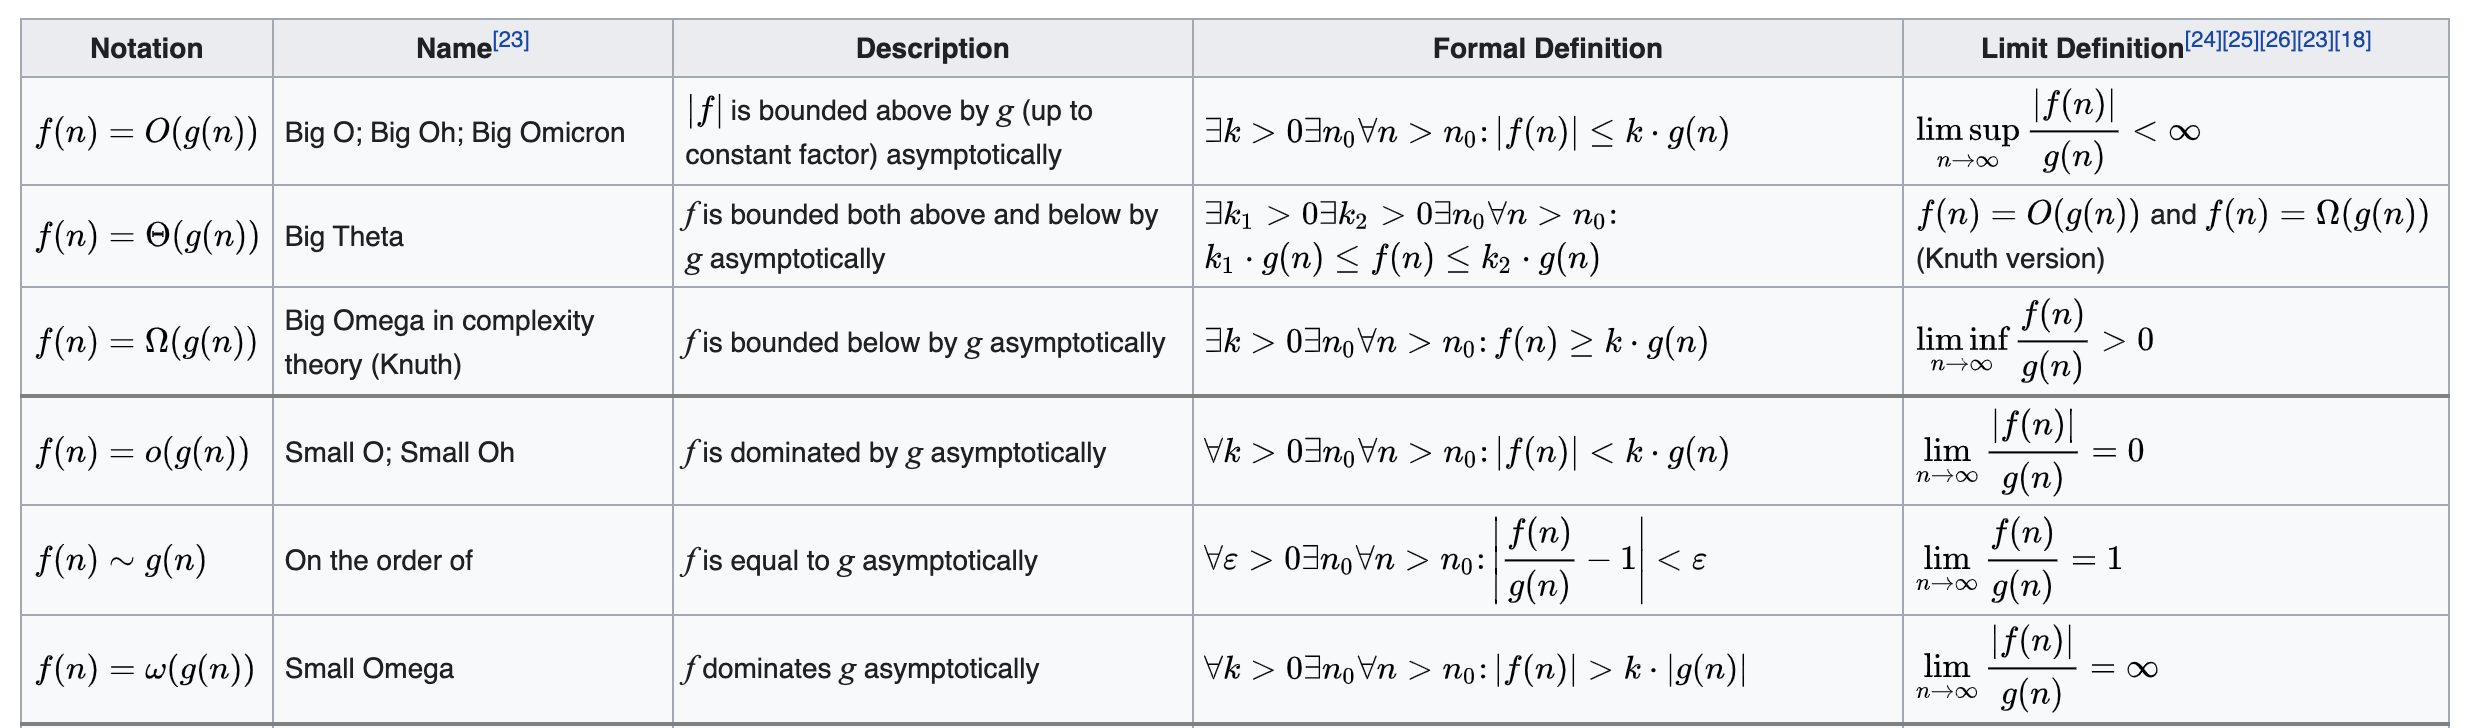
\includegraphics[width=1\linewidth]{Figs/big_o.png}
\centering
\caption{Big O notation}
		\label{un:figbigo}
\end{figure}


\section{Stirling's Approximation}
\begin{enumerate}
    \item \begin{align}
        \ln n!=n\ln n-n+O(\ln n).\label{Stirling:1}
    \end{align}
    \item \begin{align}
        \log _{2}n!=n\log _{2}n-n\log _{2}e+O(\log _{2}n).\label{Stirling:2}
    \end{align}
    \item  As $m\to \infty$, $n! = (1+o(1)){\sqrt {2\pi n}}\left({\frac {n}{e}}\right)^{n}$. In other words:
    \begin{align}
         n!\sim {\sqrt {2\pi n}}\left({\frac {n}{e}}\right)^{n}. \label{Stirling:3}
    \end{align}

\end{enumerate}
\section{Estimates of Binomial Coefficients}
We give useful bounds for Binomial coefficients: $$\binom{n}{k}=\frac{n!}{k!(n-k)!} = \frac{\prod_{j=0}^{k-1} (n-j)}{k!}$$
\subsection{Rough Upper Bounds}
\begin{enumerate}
\item A gross estimation:
\begin{align}
    \forall 0\le k \le n : \binom{n}{k}\le 2^n \label{bio:1}
\end{align}
\item Standard inequalities for upper and lower bounds:
\begin{align}
    \forall 1\le k \le n : \left(\frac{n}{k}\right)^k\le \binom{n}{k}\le \left(\frac{ne}{k}\right)^k \label{bio:2}
\end{align}
\begin{proof}
$\binom{n}{k}=\frac{n!}{k!(n-k)!} = \frac{\prod_{j=0}^{k-1} (n-j)}{k!}=\prod_{j=0}^{k-1} \frac{n-j}{k-j}\ge \prod_{j=0}^{k-1}\frac{n}{k}$ gives the lower bound. To give the upper bound, we first get $k!>\left(\frac{k}{e}\right)^k$ using induction. Assume $(k-1)!>\left(\frac{k-1}{e}\right)^{k-1}$, we then have $k!>k \left(\frac{k-1}{e}\right)^{k-1} > \left(\frac{k}{e}\right)^k$ where the second inequality has used \cref{ber:5a}. Then $\binom{n}{k}=\frac{\prod_{j=0}^{k-1} (n-j)}{k!}=\frac{n^k}{k!}\le \left(\frac{ne}{k}\right)^k$

\end{proof}
\begin{rema}
When faced with a calculation involving binomial coefficients, the bounds \cref{bio:2} often suffice to determine the correct order of magnitude of the quantity in question. 

One question: which bound better in \cref{bio:2} reflects the truth? It turns out that the answer depends on the relative sizes of $k$ and $n$.  If $k$ is small compared to $\sqrt{n}$, then $\left(\frac{n e}{k}\right)^{k}$ is the better estimate for $\left(\begin{array}{l}n \\ k\end{array}\right)$. At the other extreme, if $k=n$, then $\left(\frac{n}{k}\right)^{k}$ is exactly equal to $\left(\begin{array}{l}n \\ k\end{array}\right)$, while $\left(\frac{n e}{k}\right)^{k}=e^{n}$ even exceeds our trivial upper bound \cref{bio:1}.

\end{rema}
\end{enumerate}
\subsection{Asymptotics}
In this section we assume $n=\omega (1)$ which means $n\to \infty$.  The asymptotics will depend on how large $k$ is. By symmetry, since $\left(\begin{array}{c}n \\ k\end{array}\right)=\left(\begin{array}{c}n \\ n-k\end{array}\right)$, we may assume $0 \leq k \leq \frac{n}{2}$, which in particular implies $n-k \geq \frac{n}{2}=\omega(1)$. The upper and lower bounds in \cref{bio:2} have a difference factor $e^k$ which is not sufficient to conclude the asymptotic. 

\textbf{Case I}: $k=o(\sqrt{n})$

Here we use the representation
\begin{align*}
\left(\begin{array}{l}
n \\
k
\end{array}\right)=\frac{\prod_{j=0}^{k-1}(n-j)}{k !}
\end{align*}
Observe that
\begin{align}
n^{k} \geq \prod_{j=0}^{k-1}(n-j) \geq(n-k)^{k}=\left(1-\frac{k}{n}\right)^{k} n^{k} \geq\left(1-\frac{k^{2}}{n}\right) n^{k}=(1-o(1)) n^{k} \label{bio:4}
\end{align}
and so, for $0 \leq k=o(\sqrt{n})$,
\begin{align}
\left(\begin{array}{l}
n \\
k
\end{array}\right)=(1+o(1)) \frac{n^{k}}{k !} . \label{bio:3}
\end{align}
\begin{enumerate}
    \item If $k$ is in fact constant, then this is the best approximation one can hope for.
    \item If $k=\omega(1)$ (but still $k=o(\sqrt{n})$ ), the $k !$ term is a little inconvenient. We can replace it with an exponential expression by making use of Stirling's Approximation:
    \begin{align}
\left(\begin{array}{l}
n \\
k
\end{array}\right)=(1+o(1)) \frac{n^{k}}{k !} = (1+o(1)) \frac{1}{\sqrt{2 \pi k}}\left(\frac{n e}{k}\right)^{k} . \label{bio:3}
\end{align}
\begin{rema}
So now we can say in this case, the upper bound in \cref{ber:2} is tight up to a multiplicative $O(\sqrt{k})$-error.
\end{rema}
\end{enumerate} 

\textbf{Case II}: $k=\Omega (\sqrt{n})$

In this case we have $k=\omega (1)$. If $k \neq o(\sqrt{n})$, then we cannot get a bound as \cref{bio:3} using the above way in case I since now in \cref{bio:4} we cannot get the last equality. Instead, since now $n, k$, and $n-k$ are all tending to infinity, we can use Stirling's approximation to evaluate all three factorials. This gives
\begin{align}
\begin{aligned}
\left(\begin{array}{l}
n \\
k
\end{array}\right)=\frac{n !}{k !(n-k) !} &=(1+o(1)) \frac{\sqrt{2 \pi n}\left(\frac{n}{e}\right)^{n}}{\sqrt{2 \pi k}\left(\frac{k}{e}\right)^{k} \cdot \sqrt{2 \pi(n-k)}\left(\frac{n-k}{e}\right)^{n-k}} \\
&=(1+o(1)) \sqrt{\frac{n}{2 \pi k(n-k)}}\left(\frac{n}{k}\right)^{k}\left(\frac{n}{n-k}\right)^{n-k}  \label{bio:6}
\end{aligned}
\end{align}
In practice, $(5)$ is far too cumbersome to use. Thus, when $k$ is large, we are happy to asymptotically determine $\log \left(\begin{array}{l}n \\ k\end{array}\right)$, rather than $\left(\begin{array}{c}n \\ k\end{array}\right)$ itself.  \emph{(For example, if $f(n)\sim ae^n$, in $\log f(n)$, we will only care about $n+o(1)$ without caring what's value of the leading constant $a$ in $f(n)$.)} While this gives a less precise result, it is often much more useful. In this setting, there is a qualitative difference based on whether $k$ is comparable to $n$ or not. Note that all logarithms here are based on $2$.

\begin{enumerate}
    \item $k=o(n)$ ( of course we still have $k=\Omega (\sqrt{n})$):
    
Recall that $\left(\frac{n}{k}\right)^{k} \leq\left(\begin{array}{c}n \\ k\end{array}\right) \leq\left(\frac{n e}{k}\right)^{k}$, which gives
\begin{align*}
k \log \frac{n}{k} \leq \log \left(\begin{array}{l}
n \\
k
\end{array}\right) \leq k \log \frac{n e}{k}=k\left(\log \frac{n}{k}+\log e\right)
\end{align*}
Since $k=o(n), \frac{n}{k}$ tends to infinity, and thus the $\log e$ term is a lower-order error. Thus
\begin{align}
\log \left(\begin{array}{l}
n \\
k
\end{array}\right)=(1+o(1)) k \log \frac{n}{k} \label{bio:5}
\end{align}
In particular, the right-hand side of \cref{bio:5} is $o(n)$, which means the binomial coefficient
$\left(\begin{array}{l}n \\ k\end{array}\right)$ is subexponential (in $n$ ), i.e. $\left(\begin{array}{l}n \\ k\end{array}\right)=o(e^n)$.

\item $k=\Omega(n)$:

The story changes when $k$ is linear in $n$. Taking the logarithm of \cref{bio:6} gives
\begin{align*}
\log \left(\begin{array}{l}
n \\
k
\end{array}\right)=\log (1+o(1))+\log \sqrt{\frac{n}{2 \pi k(n-k)}}+k \log \frac{n}{k}+(n-k) \log \frac{n}{n-k}
\end{align*}
Since both $k$ and $n-k$ are linear in $n$, we can simplify the above to
\begin{align}
\log \left(\begin{array}{l}
n \\
k
\end{array}\right)=(1+o(1))\left(\frac{k}{n} \log \frac{n}{k}+\frac{n-k}{n} \log \frac{n}{n-k}\right) n=(1+o(1)) H\left(\frac{k}{n}\right) n \label{bio:7}
\end{align}
where $H(p)=-p \log p-(1-p) \log (1-p)$ is the \textbf{binary entropy function}, defined for $p \in[0,1] .$ Hence, when $k=c n$ for some fixed constant $c \in\left(0, \frac{1}{2}\right],\left(\begin{array}{c}n \\ k\end{array}\right)$ is approximately $2^{H(c) n}$. Most importantly, we see that when $k$ is linear, $\left(\begin{array}{c}n \\ k\end{array}\right)$ grows exponentially in $n$.
\end{enumerate}

\subsection{Examples}
Normally, we can apply the above conclusions like \cref{bio:3,bio:5,bio:7} to do a first analysis, and then apply Stirling's approximation to get a finer bound or order (e.g. with an improved leading constant).

\textbf{The middle coefficient}

Of all the binomial coefficients, the case when $n=2 k$ is arguably the most interesting. Recall that the trivial upper bound \cref{bio:1} gives $\left(\begin{array}{c}2 k \\ k\end{array}\right)\le 2^{2 k}$. Since there are $2 k+1$ possible sizes, that implies 
\begin{align}
    \frac{2^{2 k}}{2 k+1} \leq\left(\begin{array}{c}2 k \\ k\end{array}\right) \leq 2^{2 k}. \label{bio:9}
\end{align}
This is a bound telling more information than that given by \cref{bio:7}. 
Since from \cref{bio:7} we can only get $\left(\begin{array}{c}2 k \\ k\end{array}\right)=2^{(1+o(1))2k}$. (\uline{Please don't be confused. Of course if we apply \cref{bio:6} or even Stirling's Approximation directly, we can get a stronger bound. However when $k=\Omega(n)$, from \cref{bio:7}, we can get a rough bound easier. It's better we applied \cref{bio:7} for a rough analysis and then apply  \cref{bio:6} or Stirling's Approximation to get a finer bound.})
In fact we can view the problem as $X_1,..., X_n$ are i.i.d random variables with distribution $\mathrm {Bernoulli} \left({\frac {1}{2}}\right)$ and $\left(\begin{array}{c}2 k \\ k\end{array}\right)$ represents $2^{2k}\P\left(\sum X_i=k\right)$. 
From \cref{bio:9} we know 
\begin{align}
    \P\left(\sum X_i=k\right)=\Omega \left(\frac{1}{k}\right) \label{bio:10}
\end{align}

Below we try to improve \cref{bio:9}  (and consequently \cref{bio:10}) a little bit:

If we substitute $n=2 k$ into \cref{bio:6}, we get
\begin{align}
\left(\begin{array}{c}
2 k \\
k
\end{array}\right)=(1+o(1)) \sqrt{\frac{2 k}{2 \pi k(2 k-k)}}\left(\frac{2 k}{k}\right)^{k}\left(\frac{2 k}{2 k-k}\right)^{2 k-k}=(1+o(1))  \frac{2^{2 k}}{\sqrt{\pi k}} \label{bio:8}
\end{align}

We therefore claim 
\begin{align}
    \P\left(\sum X_i=k\right)=\Theta \left(\frac{1}{\sqrt{k}}\right) \label{bio:11}
\end{align}

From another point of viewing, since binomial distribution with $2 k$ trials and probability $\frac{1}{2}$ approximately follows a normal distribution with mean $k$ and variance $\frac{k}{2}$, or standard deviation $\Theta(\sqrt{k})$, we can get almost all sets have sizes ranging over an interval of only $\Theta \left(\sqrt{k}\right)$ \blue{need update after we include the sub-gaussian inequaltiy: 
\begin{align*}
P [|X-\mu| \geq t] \leq 2 e^{-\frac{t^{2}}{2 \sigma^{2}}} \quad \text { for all } t \in R
\end{align*}}
In other words, while there are $2k+1$ possible sizes of sets, as the most common size is $k$, we can expect $\left(\begin{array}{c}2 k \\ k\end{array}\right)$ to count a $\Theta(\sqrt{k})$ -fraction of the $2^{2 k}$ sets, which is what

\textbf{Random greedy two-colouring of hypergraphs} 

(Please ignore the name. I'm not sure what  the two-colouring of hypergraphs is.) What we want to show is to bound the following:
\begin{align}
\frac{(k-1) !(k-1) !}{(2 k-1) !} \label{bio:11}
\end{align}
To obtain an expression that is easier to work with, we shall first rewrite \cref{bio:11} in terms of a binomial coefficient, and then use our asymptotic estimates. We have
\begin{align*}
\frac{(k-1) !(k-1) !}{(2 k-1) !}=\frac{(k-1) !(k-1) !}{(2 k-1)(2 k-2) !}=\frac{1}{(2 k-1)\left(\begin{array}{c}
2 k-2 \\
k-1
\end{array}\right)}
\end{align*}
which, in light of \cref{bio:8}, shows
\begin{align*}
\frac{(k-1) !(k-1) !}{(2 k-1) !}=(1+o(1)) \frac{\sqrt{\pi(k-1)}}{2 k-1} 2^{2-2 k}=O\left(k^{-\frac{1}{2}} 2^{-2 k}\right)
\end{align*}

The same result could have been obtained by applying Stirling's Approximation to  \cref{bio:11} directly.
\begin{align*}
\begin{aligned}
\frac{(k-1) !(k-1) !}{(2 k-1) !} &=(1+o(1)) \frac{\left[\sqrt{2 \pi(k-1)}\left(\frac{k-1}{e}\right)^{k-1}\right]^{2}}{\sqrt{2 \pi(2 k-1)}\left(\frac{2 k-1}{e}\right)^{2 k-1}} \\
&=(1+o(1)) \frac{e \sqrt{\pi(k-1)}}{2 k-1}\left(\frac{k-1}{2 k-1}\right)^{2 k-2} \\
&=(1+o(1)) \frac{e \sqrt{\pi(k-1)}}{2 k-1}\left(\frac{k-1}{2 k-2}\right)^{2 k-2}\left(\frac{2 k-2}{2 k-1}\right)^{2 k-2} \\
&=(1+o(1)) \frac{e \sqrt{\pi(k-1)}}{2 k-1} 2^{2-2 k}\left(1-\frac{1}{2 k-1}\right)^{2 k-2}
\end{aligned}
\end{align*}
Since $\left(1-\frac{1}{2 k-1}\right)^{2 k-2}$ is asympotically $e^{-1}$, this matches our earlier result. \uline{However, as we can see here,
\cref{bio:8} is easier to remember than Stirling's Approximation, and, in this case at least, easier to apply.}



\bibliographystyle{IEEEtran}
\bibliography{IEEEabrv,StringDefinitions,adv_dnn}
\end{document}
